\newgeometry{top = 0.7cm, left = 1cm, right = 1cm, bottom=0.1cm}
\song{Tři oříšky (Iveta Bartošová)}
\begin{multicols}{2}
\thispagestyle{empty}

\vspace{-5px}
\ve{}
\ch{G}Marně se vlastního \ch{C}osudu ptáš\\
Co \ch{G}dnes a zítra \ch{D}schystá\\
\ch{G}Představ si, že v kapse \ch{C}oříšek máš\\
A \ch{G}ten ti dá moc \ch{D}vyzrát\\
\ch{Am}Na ty, kdo s cílem \ch{D}zlým,
\ch{G}chtějí tvou \ch{D}dráhu \ch{G}zkří\ch{G}{ž}it

\vspace{-5px}
\ve{}
Šetři si oříšky pro chvíli zlou\\
Kdy sám si náhle přiznáš\\
Život je pohádkou nedopsanou,\\
Vše stát se smí jen třikrát\\
\ch{Am}Snad ti to může \ch{D}znít, \ch{G}dnes jako \ch{D}bláznovs\ch{G}tví

\vspace{-5px}
\cho{}
\ch{G}Věř mi, že, \ch{C}to je ta na světě \ch{D}nejlepší zpráva\\
\ch{G}Pro ty, kdo uvěří \ch{Em}stane se zázrak\\
\ch{Am}Možná, \ch{C}možná, \ch{D}možná\\
Kdo jen to \ch{G}pozná, \ch{D}pozná, \ch{G}pozná\\
\ch{G}Věř mi, že \ch{C}to je ta na světě \ch{D}nejlepší zpráva\\
\ch{G}Kouzlo tří oříšků \ch{Em}křídla ti dává\\
\ch{Am}Vyhrát, \ch{C}vyhrát, \ch{D}vyhrát\\
\ch{Am}Jednou, \ch{C}dvakrát, \ch{D}třikrát

\vspace{-5px}
\ve{}
Na na na na na na......\\
\ch{Am}Snad ti to může \ch{D}znít,\\
\ch{G}dnes jako \ch{D}bláznovs\ch{G}tví

\vspace{-5px}
\cho{}


\vspace{-5px}
\re{}
\ch{G}Věř mi, že, \ch{C}království padne, když \ch{D}schází v něm láska\\
\ch{G}Chraň své tři oříšky, \ch{Em}třeba tě zázrak\\
\ch{Am}Potká, \ch{C}potká, \ch{D}potká\\
\ch{Am}Možná \ch{C}taky \ch{D}stokrát

~

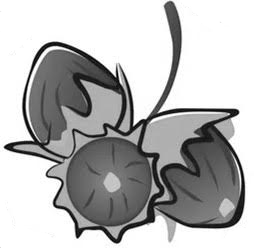
\includegraphics[width = \columnwidth]{images/tri_orisky.jpg}
\end{multicols}

\esong{}

\restoregeometry{}
